\documentclass{main}
\newcommand{\DefType}{Bachelor's Thesis} %Type of your scientific work
\newcommand{\DefTitle}{Android Bluetooth Credential Store} %Title of your work
\newcommand{\DefFirstAuthor}{Camilla Reis} %Name
\newcommand{\DefFirstAuthorMatnum}{01430500} %Matr number.
\newcommand{\DefFirstAuthorEmail}{c.reis@student.tugraz.at} %Email address
\newcommand{\DefSupervisor}{Dipl.-Ing. Dominik Ziegler} %Name
\newcommand{\DefAuthorFrontPage}{\DefFirstAuthor\\(\DefFirstAuthorMatnum)}
\newcommand{\DefAuthor}{\DefFirstAuthor}
\newcommand{\DefVersion}{1.0}
\newcommand{\DefLogo}{TU_Graz_Logo.pdf}

\begin{document}
\begin{titlepage}
%here goes titlepage

\titlesection{\DefLogo}
\newcommand{\HRule}{\rule{\linewidth}{0.5mm}} % defines a new command for horizontal lines, change thickness here
\centering
\vfill 
%------------------------------------------------
%	BS Thesis
%------------------------------------------------
\HRule\\[1cm]
{\huge\sffamily\DefType}\\[0.4cm] % Type
\HRule\\[1cm]
%------------------------------------------------
%	Android Bluetooth Credential Store
%------------------------------------------------	
\textsc{\huge\sffamily\DefTitle}\\[0.4cm]
\vfill 
%------------------------------------------------
%	Camilla Reis
%------------------------------------------------
\large{\sffamily
	\DefAuthorFrontPage\\ 	
	\href{mailto:\DefFirstAuthorEmail}{\sffamily\DefFirstAuthorEmail}\\[0.4cm]
}
\vfill
%------------------------------------------------
%	Supervisor
%------------------------------------------------
\vfill
{\large\sffamily Supervisor\\
	\DefSupervisor}
\vfill
%------------------------------------------------
%	Date
%------------------------------------------------
\vfill\vfill\vfill % Position the date down
{\normalsize\sffamily Graz, \today}





\end{titlepage}

\providecommand{\keywords}[1]{\textbf{\textit{Keywords---}} #1}

%------------------------
%	Declaration
%------------------------
\newpage
\subsection*{Statutory Declaration}
\noindent
\textit{
	I declare that I have authored this thesis independently, that I have not used other than the declared sources / resources, and that I have explicitly indicated all material which has been quoted either literally or by content from the sources used. The document uploaded to TUGRAZonline is identical to the present thesis.}
\vspace{1cm}

\subsection*{Eidesstattliche Erklärung}
\noindent
\textit{
	Ich erkläre an Eides statt, dass ich die vorliegende Arbeit selbstständig verfasst, andere als die angegebenen Quellen/Hilfsmittel nicht benutzt, und die den benutzten Quellen wörtlich und inhaltlich entnommenen Stellen als solche kenntlich gemacht habe. Das in TUGRAZonline hochgeladene Dokument ist mit der vorliegenden Arbeit identisch.}

\vspace{2cm}

\noindent
\parbox[top]{4cm}{
	\begin{center}
		\underline{\hspace*{4cm}} \\
		Date/Datum
	\end{center}
}
\hfill
\parbox[top]{6cm}{
	\begin{center}
		\underline{\hspace*{6cm}} \\
		Signature/Unterschrift
	\end{center}
} 
\newpage


%------------------------
%	Abstract
%------------------------
\begin{abstract}
\begin{adjustwidth}{65pt}{65pt}
\vspace{0.5cm}
%consise description what the thesis is about and what its contributions to the field are (what is new). Market the contributions to your readership --> mention all relevant keywords IN THE abstract!
In this paper, we explore a more secure way to share credentials over multiple devices without relying on cloud services. Sensitive data is stored on a mobile phone while accessing them over a secure Bluetooth connection. \\
It features an Android application for mobile phones and a Chrome web extension which uses the Web Bluetooth API for establishing a Bluetooth Low Energy (LE) connection between device and website. The application acts as a peripheral and advertises the data. The web extension serves as the central and reads the data after a successfully established connection. The extension then fills the read data into the login fields of the webpage. \\
To securely store sensitive information on the mobile phone it is encrypted using the symmetric-key algorithm Advanced Encryption Standard (AES) with a 256bit-generated key. The encrypted credentials are then stored using the greenDAO ORM which manages all operations of the database. The generated key lies in the Trusted Execution Environment (TEE) which is handled by the Android KeyStore and represents the most secure option for this project. \\
Assurance of authenticity of the user is reached by making use of biometric identification respectively the user's fingerprint to authenticate the sharing of the credentials.
\vspace{0.5cm} \\
\keywords{\textit{android, password manager, mobile application, aes symmetric encryption, bluetooth low energy, web extension, web bluetooth api}}
\end{adjustwidth}
\end{abstract}




\newpage
%------------------------
%	Table of Contents
%------------------------
\tableofcontents
\newpage



%-----------------------------------------------------------------------------------------
%-----------------------------------------------------------------------------------------
%	Begin of Thesis
%-----------------------------------------------------------------------------------------


%------------------------
%	Chapter 0 - Intro
%------------------------
\section*{Introduction} \label{introduction}
%Introduction into the topic; what was made; what are the problems with state of the art technology, generally a description of what was made, more like a story

Nowadays password managers are essential to our everyday lives. Studies show that the average person has up to 20 online accounts [paper] from social media, bank accounts, financial information]. As shown in [ref with passwords of people] the average user also does not create particularly safe or hard to remember the password. Also, same passwords are reused over multiple different accounts or some variation of that password. These passwords are not secure and very vulnerable to attacks. \\

However, to maintain all accounts securely many users rely on password managers to handle it for them. It makes it easier to create and remember multiple passwords, which are different from each other but at the same time equally safe. There are different kinds of password managers. Some store the data locally, for example on a computer or mobile device. It is a safe way to manage credentials but making them accessible throughout different devices can be challenging. In order to make them available on multiple devices, some of those password managers offer the possibility of cloud synchronization. This may be very convenient when working on different devices but not very reliable when it comes to the security of data. The risks are data being corrupted, stolen or wiped. [https://www.bbc.com/news/business-36151754] [paper attack on cloud services]. Then there are password managers that are entirely cloud-based meaning that no data is saved locally on any device and credentials are accessed over a website. Also, some password managers support browser integration which makes passwords accessible through the browser in use. By uploading sensitive data in any form onto the internet, the risk of an attack may increase.
The goal is to store credentials as safely as possible and to make them available on different devices while at the same time without relying on any cloud services. \\

In this project, an Android credential manager is designed that does not store data onto the internet but rather shares them through a secured Bluetooth Low Energy (LE) connection established with a Chrome extension using the Web Bluetooth API [ref web Bluetooth API google link]. The data is stored on the device and only on demand one selected credential pair consisting username and password is shared with the extension at a time. Accessing and sending credentials requires authentication from the user in the form of biometric information or a master password. It is guaranteed that only the owner of the mobile phone can access and share his credentials. The Web Bluetooth API [chome API link] on the other hand receives the data that is sent from the Android application and fills them in into the text fields on the website. Neither is it necessary to type in the credentials manually nor even make them visible. \\ 
%explain more the extension and web Bluetooth API ?? https://developers.google.com/web/updates/2015/07/interact-with-ble-devices-on-the-web)\\

This paper consists of 8 chapters that are structured as follows: Section \ref{motivation} shows the motivation behind this project, while section \ref{relwork} explains related work that has already been done on this subject. Section \ref{architecture} handles the architecture of the project and presents the topics in detail. Section \ref{seceval} illustrates a brief security evaluation with common criteria, and section \ref{bluetooth} discusses Bluetooth, and it's underlying security. Furthermore, section \ref{limitations} describes the limitations that apply to this project and future work is explained in section \ref{futurework}. Finally, the conclusions are drawn in section \ref{conclusion}.




%------------------------
%	Chapter 1
%------------------------
\section{Motivation} \label{motivation}
The motivation of this project is to provide a safe possibility for mobile phones to store credentials that are available to the user on multiple devices without cloud storage.

%Poster session motivation
There exist many applications that offer the service to store user credentials safely. To synchronize data between multiple devices they rely on cloud services where data confidentiality cannot be guaranteed.
Mobile phones offer a secure way to store data, for example through hardware-backed key storage.
By relying on this technology, we can provide secure data storage for user credentials. 

%------------------------
%	Chapter 2
%------------------------
\section{Related Work} \label{relwork}
papers on similar topics

PWM local w/ possible cloud sync
PWM cloud based 
both types support browser integration

Or just browser itself offers to store credentials for the next time loging into the website.

password managers that rely on cloud services

password managers that are integrated into web service, google pw managaer, firefox, ...

security issues e.g. last pass had leaks in their release.


MAYBE put to related work which decisions we made, which cipher, which encryption method, ...??


%------------------------
% Chapter 3
%------------------------
\section{Architecture of Project} \label{architecture}
%generall description about the technologies used in the project and how they interact, also why I used the technologies (advantages and disadvantages); also insert figures of the app and throughout this chapter more of each specific activity
As mentioned above, we decided to implement an Android application for mobile phones to store sensitive data on it. Since the Chrome browser offers an interface for using Bluetooth LE on the web, we decided to develop a Chrome extension to utilize their Web Bluetooth API. [link] \\

The API initiates the connection upon a button click from the user and searches for BLE devices that are near and offer a specific service that is defined through a UUID, a universally unique identifier. Once paired with the mobile app, the secure Bluetooth connection has been established, and the transmission of data can take place. Upon successful pairing, the extension is allowed to read characteristics that are advertised on the app. The characteristics contain the values of username and password, which the extension inserts directly into the login fields of the website. \\

\noindent First, the requirements of the application as well of the extension were defined: \\

\noindent Application requirements:
\begin{itemize}
\item Safe storage of credentials (account name, username, and password)
\item Adding, changing and deleting credentials
\item En- and decryption of data 
\item Authentication through biometric identification
\item Establishing a Bluetooth connection with the web extension
\end{itemize}
\vspace{0.3cm}
\noindent Extension's requirements:
\begin{itemize}
\item Injection of a button onto the website to establish a Bluetooth connection
\item Reading the advertised characteristics
\item Filling credentials into the proper login fields
\end{itemize}


%technical details:
\noindent For convenience purposes, we implemented the application for API level 23 minimum and up using Android Studio as the IDE. To go more into detail about the app, it consists of a MainActivity.java [ref figure 1], which contains four different menu items: \textit{Accounts}, which provides the user with an interface to manage their login accounts; \textit{Connection}, where users can establish the Bluetooth connection and send their login data to the web browser; \textit{Settings} and \textit{About}. We will go more into detail about the functionality of the activities \textit{Accounts} and \textit{Connection}. Subsequently, we will examine how the application handles data storage, encryption, and authentication in greater detail. \\

\begin{figure}[H]
\centering
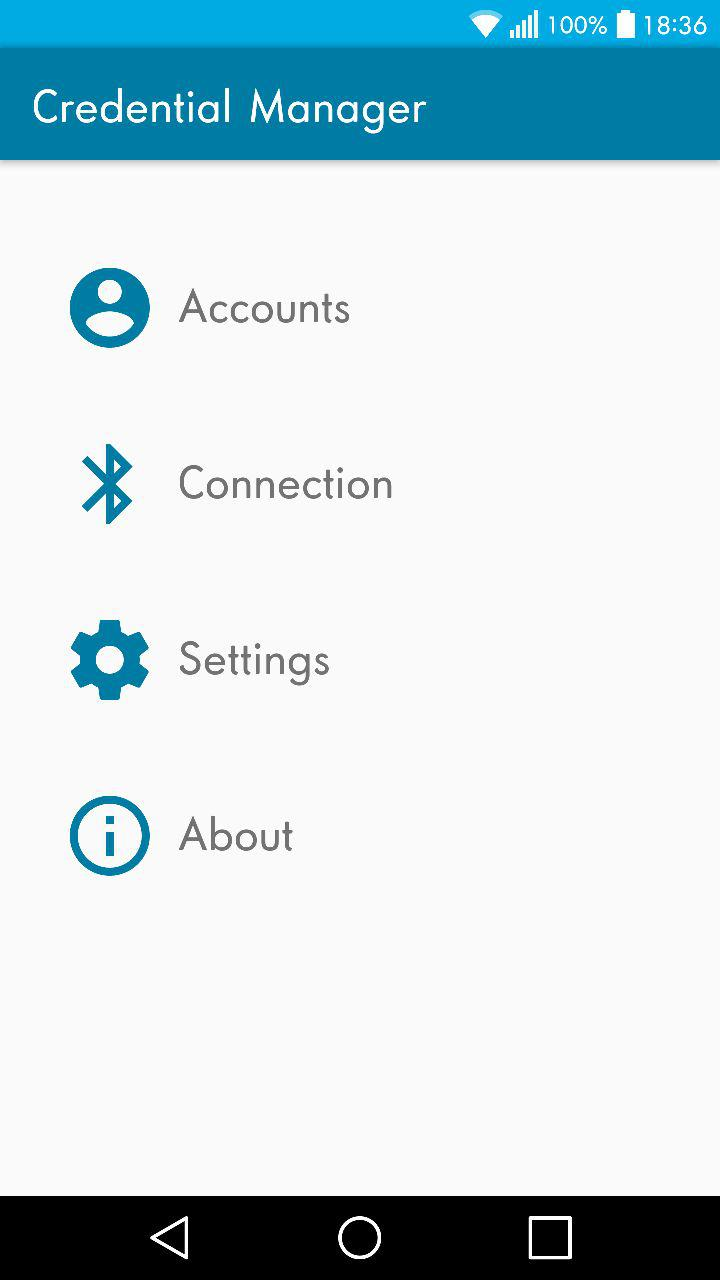
\includegraphics[width=6cm]{images/MainActivity}
\caption{MainActivity, which is shown at start up of the app}
\label{fig:mainactivity}
\end{figure}

\subsection{Activity \textit{Accounts}}
By clicking on the menu item \textit{Accounts}, the user is asked to authenticate themselves using biometric information in the form of fingerprint or a master password as seen in figure \ref{fig:authentication}\protect\subref{auth_screen}. Upon successful verification, the interface is shown where the user has an overview of his saved credentials as seen in Figure \ref{fig:accountactivity}\protect\subref{show_acc}. By clicking the floating action button on the bottom right of this interface, the activity is switched to the \textit{AddAccountsActivity}, where the user can add a new login account as seen in Figure \ref{fig:accountactivity}\protect\subref{add_acc}. Here the user types in the website where credentials belong to as well as the username and password itself. Clicking the \textit{SAVE}-button encrypts and adds the credential to the database. \\

When clicked on one of the existing credentials in the list, it takes the user to the interface shown in Figure \ref{fig:accountactivity}\protect\subref{change_acc}.  Here the values can be changed and saved again, or the login account can be deleted from the database. When deleting a credential, the user will be asked via a prompt as seen in Figure \ref{fig:accountactivity}\protect\subref{prompt_delete}.

\begin{figure}[H]
\centering
\subfloat[ShowAccountActivity, which is shown after authentication]{{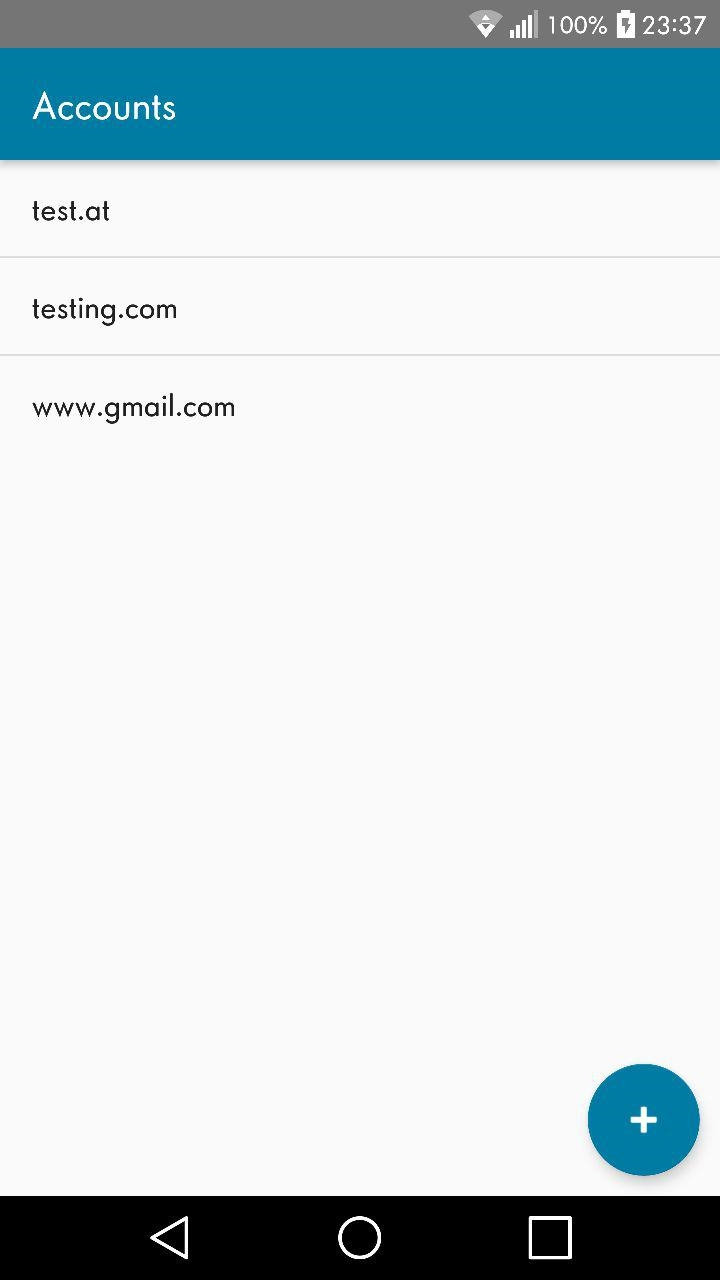
\includegraphics[width=4cm]{images/ShowAccountsActivity}\label{show_acc} }}
\qquad
\subfloat[AddAccountActivity, which is shown after clicking the floating action button on the bottom right corner]{{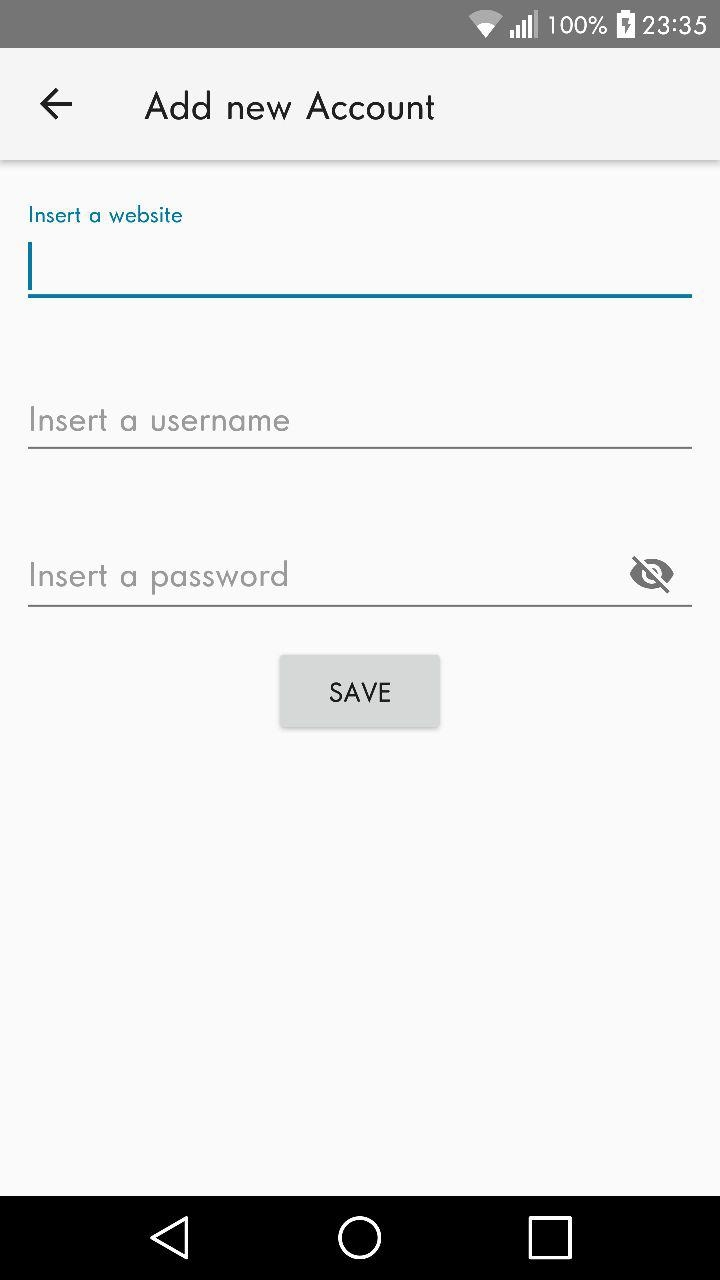
\includegraphics[width=4cm]{images/AddAccountActivity}\label{add_acc} }}
\qquad
\subfloat[ChangeAccountActivity, which is shown when clicked on a existing credential in the list]{{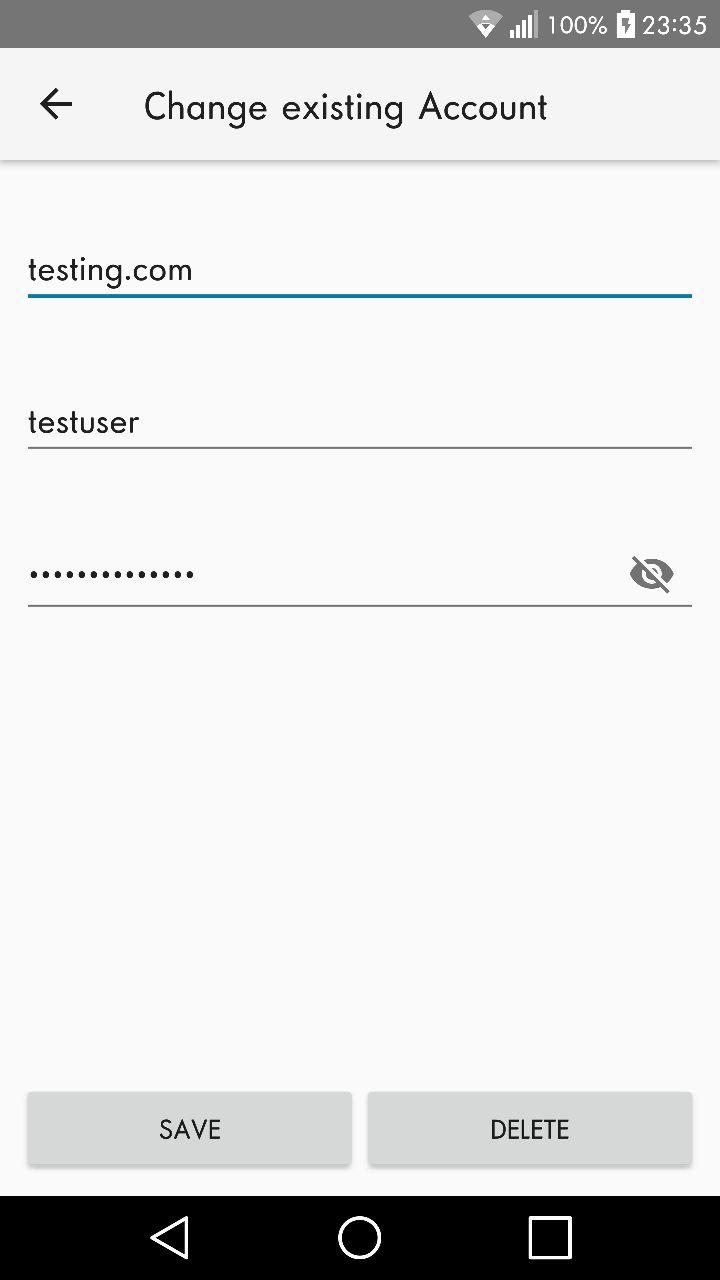
\includegraphics[width=4cm]{images/ChangeAccountActivity}\label{change_acc} }}
\qquad
\subfloat[Asking the user before deleting the credential out of the database]{{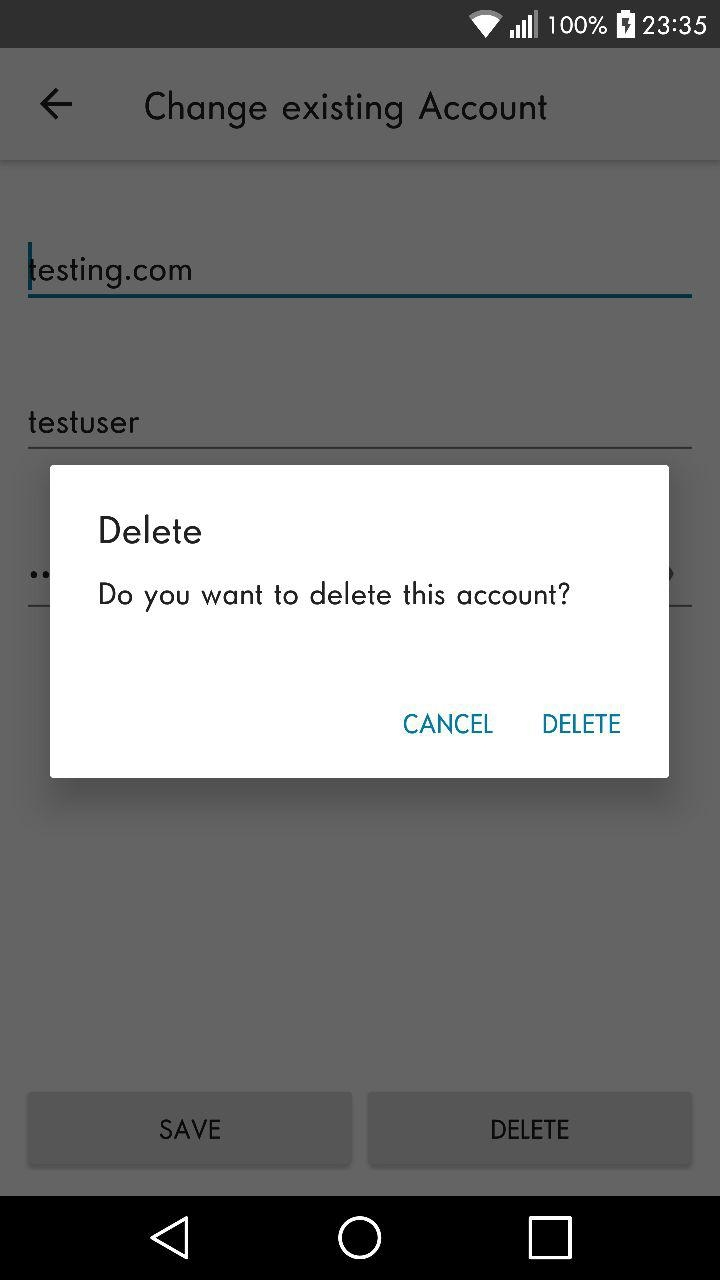
\includegraphics[width=4cm]{images/DeleteAccount}\label{prompt_delete} }}
\caption{Activity \textit{Accounts}}
\label{fig:accountactivity}
\end{figure}



\subsection{Activity \textit{Connection}}
After selecting the menu item \textit{Connection}, the app checks immediately if Bluetooth is enabled and if not it prompts the user to allow turning on Bluetooth on the mobile phone as shown in Figure \ref{fig:connectionactivity}\protect\subref{prompt_bt}.
If the activation is denied, then the application will return to the main activity with an error message saying "\textit{Bluetooth is Not Enabled}" which is shown in Figure \ref{fig:connectionactivity}%\protect\subref{bt_notEnabled}. \\
. \\

Once Bluetooth is enabled, the accounts, which are available to share over the BLE connection to the web browser, are listed.
At first, the application does not advertise. The user is asked to select an account that he wants to send to the Web Bluetooth API for login as seen in Figure \ref{fig:connectionactivity}\protect\subref{not_advertising}. Before the credentials are shared, the user is asked to authenticate himself again using his fingerprint or his master password. Figure \ref{fig:connectionactivity}\protect\subref{advertising} shows that only after successful authentication the advertising starts and the Web Bluetooth API searches for BLE devices that are near.

\begin{figure}[H]
\centering
\subfloat[Prompt to enable bluetooth]{{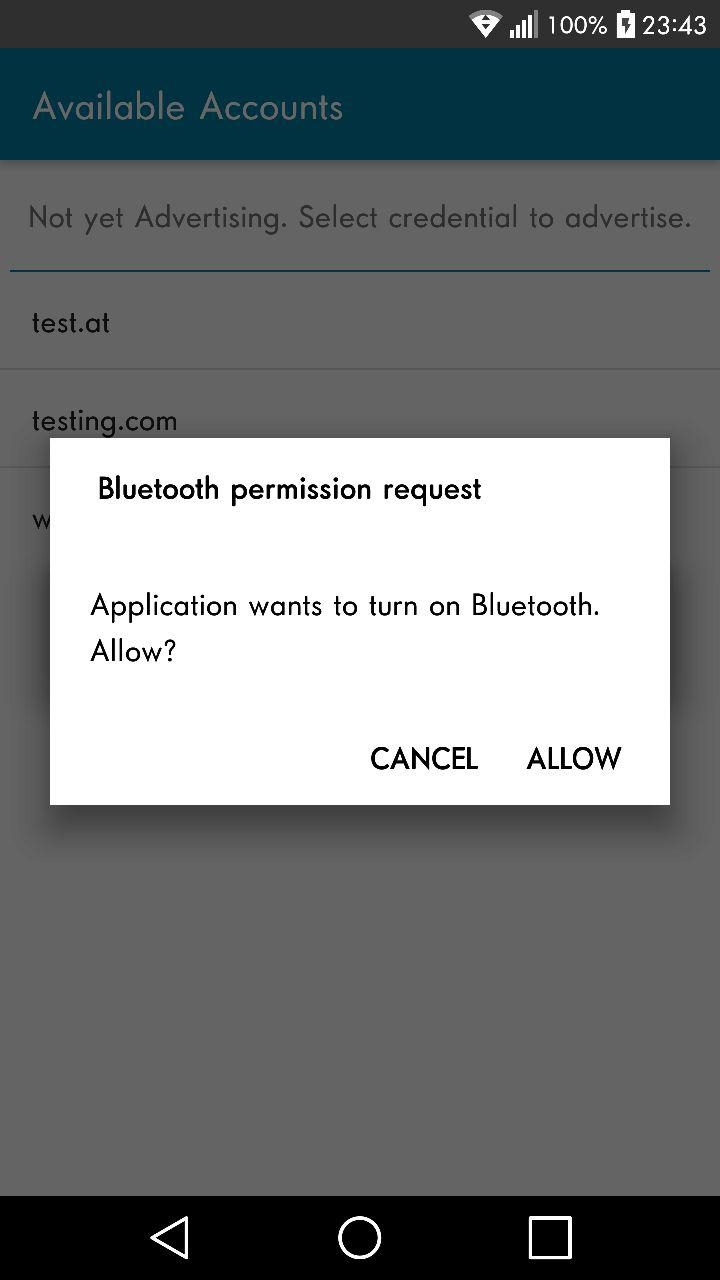
\includegraphics[width=4cm]{images/BT_english}\label{prompt_bt} }}
\qquad
\subfloat[screenshot not advertising, please select credential]{{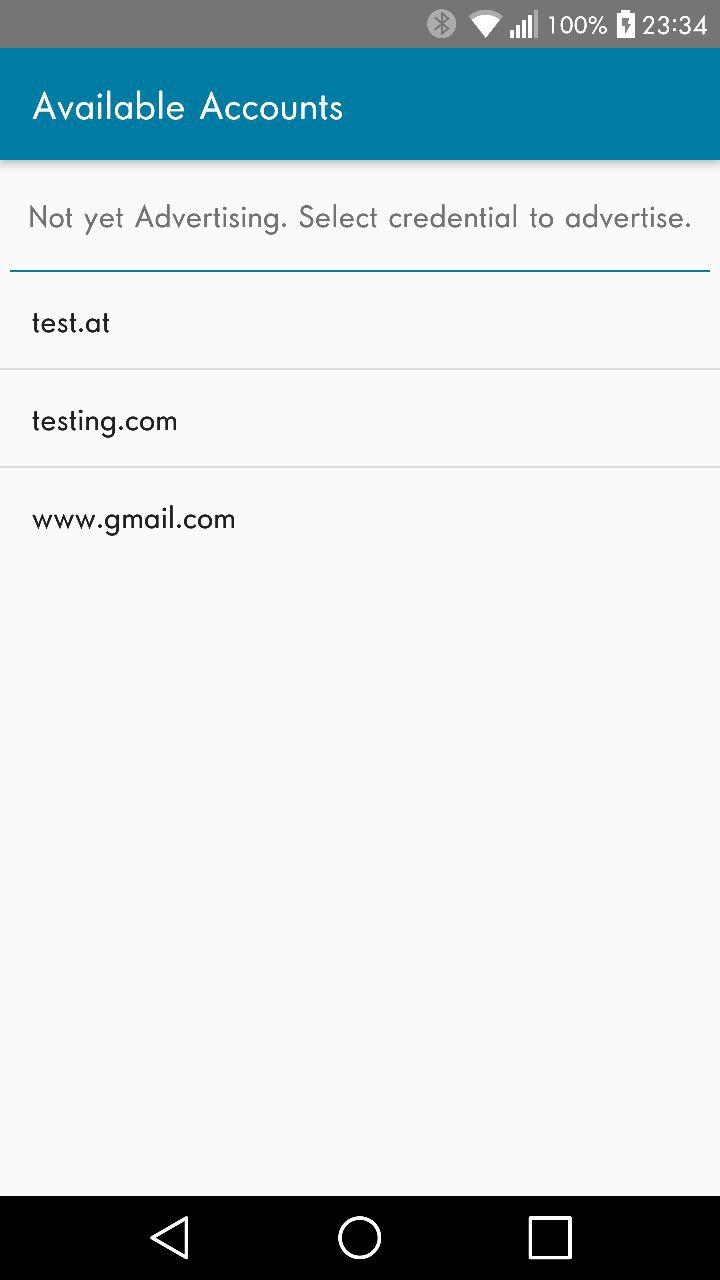
\includegraphics[width=4cm]{images/AvailableAccounts}\label{not_advertising} }}
\qquad
% !!!!!!!!!!!!! change jpg once programming done and working!
\subfloat[screenshot of now advertising, please keep screen on]{{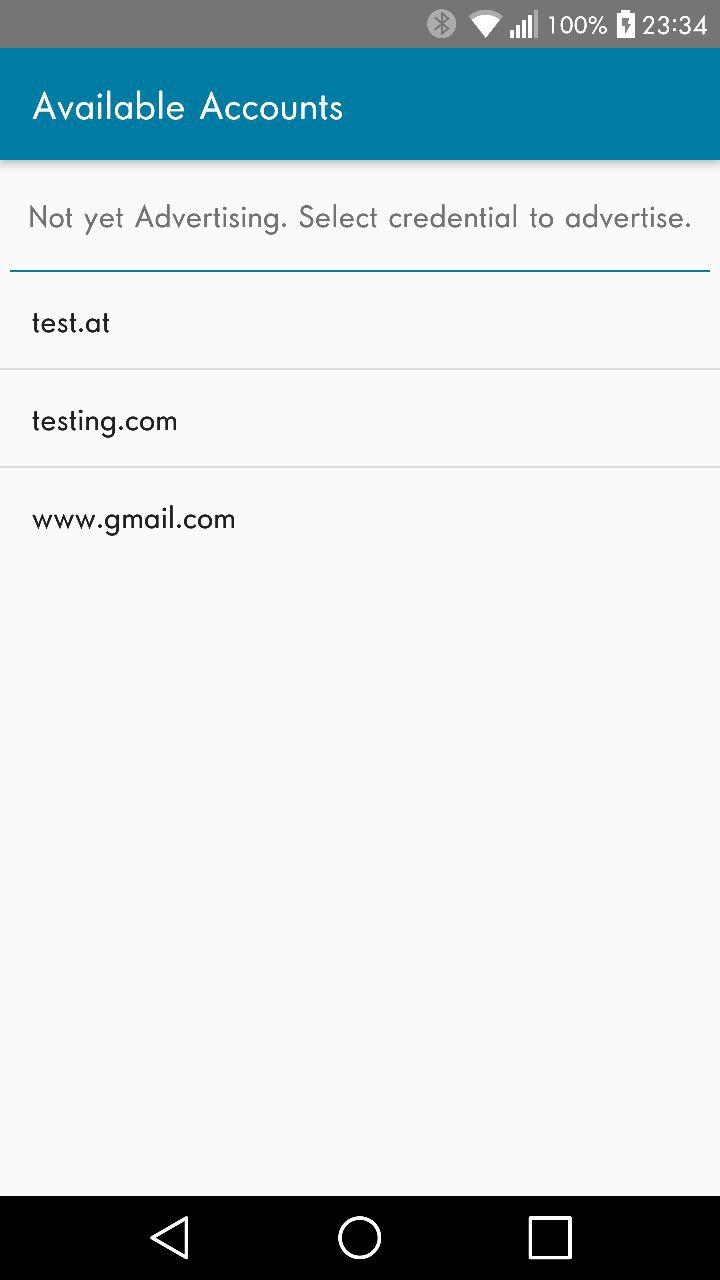
\includegraphics[width=4cm]{images/AvailableAccounts}\label{advertising} }}
%\qquad
%\subfloat[Asking the user before deleting the credential out of the database]{{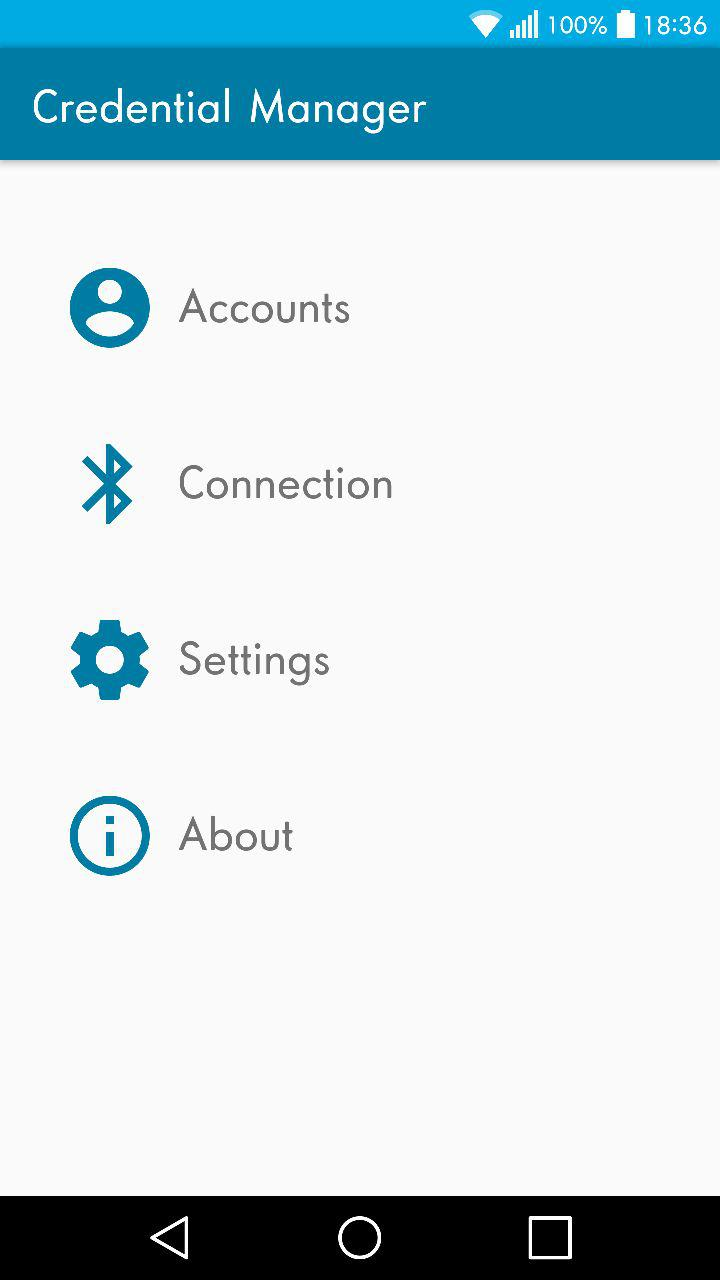
\includegraphics[width=5cm]{images/MainActivity} }}
\caption{Activity \textit{Connection}}
\label{fig:connectionactivity}
\end{figure}




\subsection{Storage of Credentials using the greenDao ORM}
Since the goal is to store user credentials on the phone,  we need a suitable database structure. One option is using a common SQLite database, which is mostly used for Android applications. SQLite databases use, as conventional SQL databases, SQL queries to store, retrieve and delete data. SQL queries are vulnerable to security attacks, for example, second-order SQL injections. A SQL injection is defined by a ... [Detection of SQL Injection Attacks]. This kind of attack increases the risk of storing data safely and may lead to a vulnerable application.\\
Another argument against a traditional SQLite database is the writing of SQL can be time consuming.

For this project, we decided not to use SQLite but instead an object/relational mapping which handles SQL processes for us.\\
To manage the tasks of storing, deleting, updating and querying a so-called \textit{object/relational mapping} is used to save time and resources. We decided on the greenDAO ORM [ref http://greenrobot.org/greendao/] as it has an overall good performance and saves time because it does not require as much programming effort compared to other frameworks as discussed in [ref greendao]. 



%IDEA: maybe split up the encryption and the hardware backed keystore, since it is so much information??
%\subsection{Encryption of Data with hardware-backed Android KeyStore}
\subsection{Encryption of Data}
%just explaining the en and decryption of data, all about choosing a key: all about cipher and algorithm, code lines and android developer cites, modes paddings usw.
For en- and decryption of the sensitive user credentials there are some different possibilities out there. One option of storing passwords is hashing the password and storing that hash instead of the password into the database. Some hash algorithms are SHA256 or SHA512 as mentioned in [Implementation and Performance Analysis of PBKDF2]. But as also stated in the paper, these passwords can be recovered by multiple different attacks such as Brute Force or Dictionary attack.
Another way to store sensitive data is to hash it with a random string of bits, called a \textit{salt}, attached to the password which is then saved with the hash of the password. This can also become vulnerable to the Dictionary Attack as stated in [https 3 wrong ways to store a password].
Nowadays it is common to use a key derivation function to safely store password such as the \textit{password-based key derivation function 2 (PBKDF2)} [ref pbkdf2 secure for passwords]
The problem which arises is that the strength of the encryption will depend on the password chosen by the user. As mentioned above more than 90\% of users chose a password that is between 6 and 9 characters long, and most of them do not include non-alphabetical characters, meaning it would take less time to retrieve the password through some attack. [ref 3 wrong ways]. Therefore, we need a way to guarantee safe en- and decryption without depending on the user's ability to create a secure password. \\

As for this project we chose to rely on the hardware-backed Android KeyStore to generate a 256bit key. To create a key that is then used for en- and decrypting data, we implemented an instance of the Android Keystore. In \cite{androidkeystore} it is stated that the Android Keystore provider lets the individual app store and manage its own credentials while making sure no other application can access them. 


The algorithm used to generate the secret key is the AES algorithm. The key is used for encryption as well as decryption. explain aes algorithm. We decided to go with a symmetric algorithm for various reasons: the algorithm is much faster than an asymmetric algorithm which makes it less expensive but especially because there is no need for distribution of a public encryption component. All encryption happens in the background on the phone.
As for the mode of the cipher we used a GCM block cipher. explain block cipher, explain gcm: deterministic algorithm, operation on fixed length groups of bits called blocks.
used aes/gcm/no padding, supported from 23 and above, and supports only 12 byte long IVs
change IV so a random string which is created with an own securerandom, explain secure random, link from android website
set that keyspecbuilder takes my own created IV with setting (look up in code) this line to "false". this means that android allowed the usage of an own IV instead of relying on their own, since they think the developer is not secure enough (search link that IV cipher get IV is not secure enough --> book). explicitely set the key to use own secure random as the IV.

after the key is built, can be stored away and is retrieved using an alias. an alias is an identifier that refers to the key that is stored in the TEE. the key never leaves the trusted environment and all encryption operations are done in the background.


as mentioned, the key is stored in the Trusted Execution Environment (TEE). The TEE is... paper The TEE is supported by the device manufacturer and represents the most secure option to store the encryption key. the tee is supported by the device. as for all android device that have an qualcomm CPU the tee is supported. paper 


\cite{ahmad2013enhancing} \cite{cooijmans2014analysis}


\subsection{Hardware-backed Keystore}
explain hardware-backed keystore, and android keystore, that android with qualcomm cpu implements the tee. securest way to store keys, never leaves the environment (paper)
what does hardware backed mean.
and tee
how does the android keystore play its role, only can use android key store if device is secured. meaning if device is looked using a pattern, lock, etc or fingerprint. if device is not locked then it is easy to retreive the .... what?
lock screen must be set in order to use key.
this is done with the class KeyguardManager. The KeyguardManager ...dev site android cite




\subsection{Authentication through Biometrics}
To securely protect the access and sending of user credential the app uses biometric authentication in the form of fingerprint scanning. The application does not store any biometric user information in a database. Rather it retrieves the already saved fingerprints on the Android mobile phone. This way it ensures that only the owner of the mobile phone has access to the credentials and the app does not have to handle the storage of the biometric information.

The application checks if the saved fingerprints contain the one that the user scanned and returns a successful authentication. Otherwise, it throws an error saying that the authentication failed.  If the phone does support fingerprint scanning, but there are no fingerprints stored on the device, the application returns an error message saying that the user must save at one fingerprint onto the device. If the phone does not have a fingerprint sensor to support scanning mechanism the user has the option of entering a master password, which is set upon the first usage of the application. 

As mentioned above, upon every request to send an account login the user has to reauthenticate using his fingerprint or a master password before sharing credentials with the Web Bluetooth API. This security mechanism would prohibit unwanted distribution of sensitive data if the user left their phone unattended with the application still running.


%we ref to auth screen in Figure \ref{fig:authentication}\protect\subref{auth_screen}.

\begin{figure}[H]
\centering
\subfloat[Activity where user is asked to auhenticate themselves using either his fingerprint or a master password]{{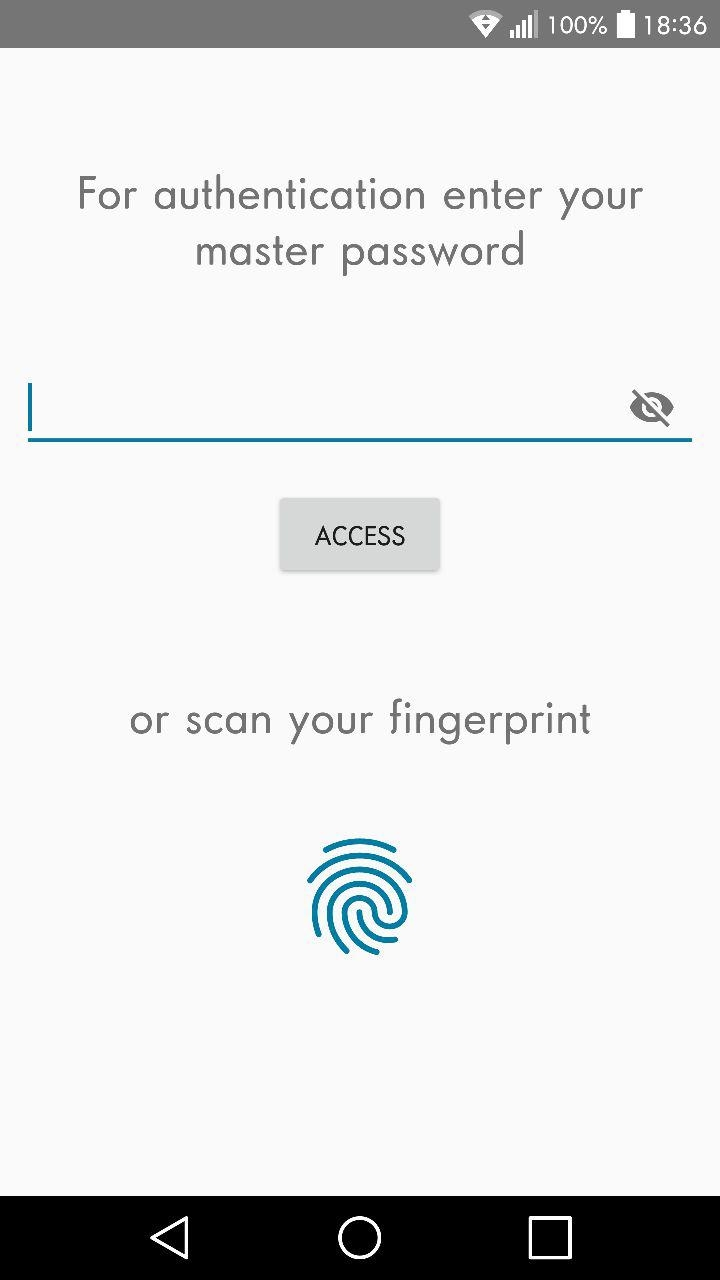
\includegraphics[width=4cm]{images/AuthenticationScreen}\label{auth_screen} }}
\qquad
%!!!!!!!!!!!!! change to on authentication failed
\subfloat[On Authentication failes]{{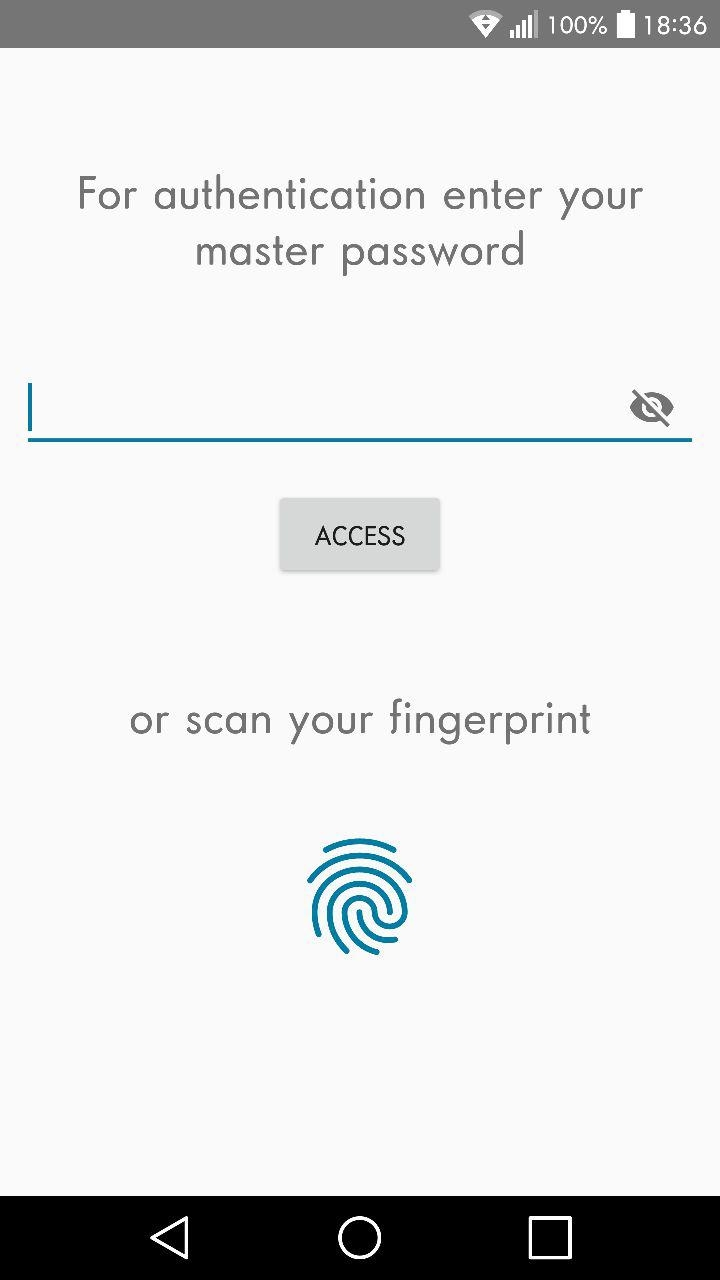
\includegraphics[width=4cm]{images/AuthenticationScreen}\label{auth_fail} }}
\caption{Authentication with fingerprint: In \protect\subref{auth_screen} you see a screen.}
\label{fig:authentication}
\end{figure}

\subsection{Peripheral and Central roles}
Usually, the Android application has the central role in a Bluetooth LE connection, for example when communicating with Bluetooth LE devices, such as a heart rate monitor or beacon. Therefore, the app serves as the client while the Bluetooth LE device acts as the server, sending data that the application wants to receive.

In this scenario, however, the Android app serves as the server, where it advertises the data that the Bluetooth LE extension wants to read. Consequently, the application opens a GATT server to advertise the characteristics and the extension, on the other hand, acts as the client and retrieves those advertised characteristics from the app. The extension implements a GATT service and reads the values from the characteristics, which are the login credentials.


%------------------------
% Chapter 4
%------------------------
\section{Security Evaluation with Common Criteria} \label{seceval}
%eher kurz gehalten
see how to conduct a security evalutation of an android app, list all common criteria, maybe make a table??


%------------------------
% Chapter 5
%------------------------
\section{Bluetooth and it's Security} \label{bluetooth}
generall structure of bluetooth low energy and why bluetooth low energy was chosen.
section about security of bluetoothLE and security concerns that may arise when using the app
writing first about how a resriction it was to not use classic bluetooth, also refer to next chapter.

(papers about ble being unsafe)


%------------------------
% Chapter 6
%------------------------
\section{Limitations of Application} \label{limitations}
In this section, some encountered limitations are discussed since they have not been established yet due to necessary technological progress of components or infeasibility. \\

\subsection{Bluetooth LE instead of Bluetooth Classic}
For the connection, we chose Bluetooth LE since the Chrome Web Bluetooth API can only support Bluetooth LE at the moment. Although as mentioned earlier, Bluetooth LE  can limit the security, it can be a task for future work to encrypt the communication channel further by using asymmetric encryption. ??? \\

\subsection{Security decreases with root privilege}
When the device is rooted, the security of the user credentials cannot be guaranteed anymore. As stated in [oncerootalwaysthreat], the Android permission system is one of the most important security mechanism for protecting critical system resources on Android phones. Before an application can access resources, it needs certain permissions which are granted by the Android permission system. The application asks for permission with check functions and if it is granted the application programming interface (API) returns \textit{PERMISSION\_GRANTED}, or in case of denial, it returns \textit{PERMISSION\_DENIAL}. \\
Root privilege on an android phone is the highest privilege in user mode and does not need any further permissions from the system to gain access to sensitive data or hardware interfaces, which leads to high risk in security when storing private data. Hence, Android's Shared Preferences and SQLite databases become accessible as mentioned in [Vulnerability Detection in Recent Android Apps]. Therefore, it is not possible for rooted devices to provide a safe possibility to store user credentials. \\


%------------------------
% Chapter 7
%------------------------
\section{Future Work} \label{futurework}
This section presents ideas that could be actualized in the near future once the necessary technology has progressed. These features are not part of the scope of this project and therefore have not been implemented further since they may be quite time-consuming to realize or not possible with start-of-the-art technology. \\


\subsection{Bluetooth Classic instead of Bluetooth Low Energy}
If in the future the API also supports the implementation of Bluetooth classic, maybe switch to BT classic? \\
maybe more secure, no advertising. maybe better for sending back information? --> research

\subsection{Encryption of BLE connection}
Encrypt Bluetooth LE connection of phone and web API with own encryption keys for a safer communication channel. BLE unsafer [ref paper with low energy comes low security], paket sniffer can read out all data in plain text that is sent over a ble connection. \\

\subsection{Encryption of tables}
Encrypt the tables with bcrypt to provide higher security. although key cannot be retrieved from the TEE to decrypt the data in the database, but to create a safer environment it is possible to decrypt the entire table with scrypt/bcrypt.\\

\subsection{Implementation of password generator}
Implementation of a password generator in the application to increase the convenience for users to create safer passwords. generate passwords that use special characters, letters and numbers and that are more than 20 characters long. \\


\subsection{Creating account from the broswer}
Create new login credentials and send them back to the application for storage. not only sending password to the website but also while creating a new account for a website user can select an option to send those newly created credentials back to the application to securely save them on the device. \\






%------------------------
% Chapter 8
%------------------------
\section{Conclusions} \label{conclusion}
Very short summery of project, maybe 300-400 words




%------------------------
% Resouces
% F11 to build compile again with F1, build again F5
%------------------------

\bibliographystyle{ieeetr}
%put here file name
\bibliography{references}


\end{document}
